% Part: conditional-logics
% Chapter: minimal-change-semantics
% Section: true-false

\documentclass[../../../include/open-logic-section]{subfiles}

\begin{document}

\olfileid{con}{min}{tf}

\olsection{Truth and Falsity of Counterfactuals}

A counterfactual $!A \cif !B$ is (non-vacuously) true if the closest
$!A$-worlds are all $!B$-worlds, as depicted in \olref{fig:true}.

\begin{figure}
\begin{center}
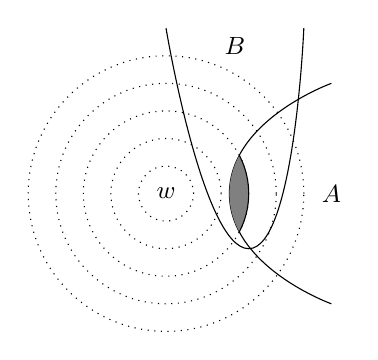
\begin{tikzpicture}[scale=.7]\small
  \draw[dotted] (0,0) node {$w$} circle (.5) circle (1)
  circle (1.5) circle (2) circle (2.5);
  \begin{scope}
    \draw[clip] plot [smooth,tension=1.2] coordinates { (3,2) (1.15,0) (3,-2)};
    \filldraw[fill=gray] (0,0) circle (1.5);
  \end{scope}
  \draw plot [smooth,tension=1.2] coordinates {(0, 3) (1.5,-1) (2.5,3)};
  \path (1.25,3) node[below] {$\formula{B}$};
  \path (3,0) node {$\formula{A}$};
\end{tikzpicture}
\caption{True counterfactual}
\ollabel{fig:true}
\end{center}
\end{figure}

It can be false in two ways. One way is if the closest $!A$-worlds are
not all $!B$-worlds. In this case, $!A \cif \lnot !B$ is also false
(see \olref{fig:false}).

\begin{figure}
\begin{center}
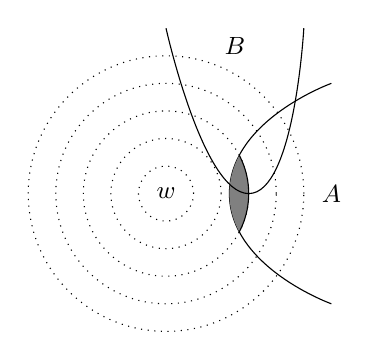
\begin{tikzpicture}[scale=.7]\small
  \draw[dotted] (0,0) node {$w$} circle (.5) circle (1)
  circle (1.5) circle (2) circle (2.5);
  \begin{scope}
    \draw[clip] plot [smooth,tension=1.2] coordinates { (3,2) (1.15,0) (3,-2)};
    \filldraw[fill=gray] (0,0) circle (1.5);
  \end{scope}
  \draw plot [smooth,tension=1.2] coordinates {(0, 3) (1.5,0) (2.5,3)};
  \path (1.25,3) node[below] {$\formula{B}$};
  \path (3,0) node {$\formula{A}$};
\end{tikzpicture}
\caption{False counterfactual, false opposite}
\ollabel{fig:false}
\end{center}
\end{figure}

If the closest $!A$-worlds do not overlap with the $!B$-worlds at all,
then $!A \cif !B$. But, in this case all the closest $!A$-worlds are
$\lnot !B$-worlds, and so $!A \cif \lnot !B$ is true (see
\olref{fig:false-opposite}).

\begin{figure}
\begin{center}
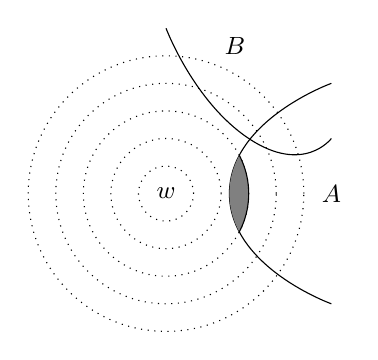
\begin{tikzpicture}[scale=.7]\small
  \draw[dotted] (0,0) node {$w$} circle (.5) circle (1)
  circle (1.5) circle (2) circle (2.5);
  \begin{scope}
    \draw[clip] plot [smooth,tension=1.2] coordinates { (3,2) (1.15,0) (3,-2)};
    \filldraw[fill=gray] (0,0) circle (1.5);
  \end{scope}
  \draw plot [smooth,tension=1.2] coordinates {(0, 3) (1.5,1) (3,1)};
  \path (1.25,3) node[below] {$\formula{B}$};
  \path (3,0) node {$\formula{A}$};
\end{tikzpicture}
\caption{False counterfactual, true opposite}
\ollabel{fig:false-opposite}
\end{center}
\end{figure}
\end{document}
